\documentclass[11pt]{article}
\usepackage[margin=1in]{geometry}
\usepackage{amsmath, amssymb, amsthm, esint}
\usepackage{fancyhdr}
\usepackage{tikz, tikz-3dplot}
% \usepackage{hyperref}
\usepackage{enumitem}
\usepackage{float}
\usepackage{cancel}

\pagestyle{fancy}
\fancyhf{}
\setlength{\headheight}{14pt}
\lhead{Miscellany}
\cfoot{\thepage}

\begin{document}
\begin{center}
    \tableofcontents
\end{center}
\setcounter{page}{1}
\newpage
\section{Zero Forcing Game}
\subsection{The game itself}
The set of linear equation 
$\begin{cases}
    ax+by=0\\
    a\neq 0, y= 0
\end{cases}$ implies that $x=0$. We can generalize these condition to: 
\[
    \begin{cases}
        a_1x_1+a_2x_2+\dots+a_nx_n\\
        a_1 \neq 0 \, \& \, a_i = 0 \text{ for } i \geq 2
    \end{cases}
\]
\subsection{Trun into Graph}
\vspace{10pt}
\begin{minipage}{.3\textwidth}
    \centering
    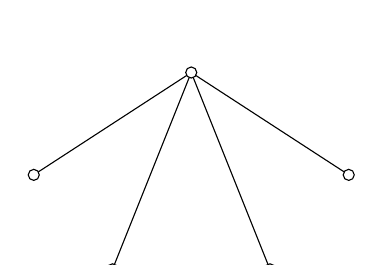
\begin{tikzpicture}
        % \tikzset{point/.style={circle,draw,fill=white,inner sep=1.5pt}}
        % \node[point] at (A) {};
        \coordinate (A) at (-2, .7);
        \coordinate (B) at (-1, -.5) ;
        \coordinate (C) at (1, -.5);
        \coordinate (D) at (2, .7);
        \coordinate (E) at (0, 2);

        \draw[black] (A)--(E);
        \draw[black] (B)--(E);
        \draw[black] (C)--(E);
        \draw[black] (D)--(E);

        \filldraw[fill=white,draw=black] (A) circle (2pt);
        \filldraw[fill=white,draw=black] (B) circle (2pt);
        \filldraw[fill=white,draw=black] (C) circle (2pt);
        \filldraw[fill=white,draw=black] (D) circle (2pt);
        \filldraw[fill=white,draw=black] (E) circle (2pt);
    \end{tikzpicture}
\end{minipage}
\hfill
\begin{minipage}{.6\textwidth}
    \vspace{0pt}
    \textbf{Coloring Rules}
    \begin{enumerate}
        \item If a black vertex has exactly one white neighbor, then the white neighbor is forced to be black.
        \item Repeat until no more changes occur.
    \end{enumerate}
\end{minipage}
\subsection{The Adjacency Matrix}
Let $G = (V,E)$ with $V = \{v_1, v_2, \dots, v_n\}$. The \textbf{Adjacency Matrix} $A=(a_{ij})$ of $G$ is
\[
    a_{ij} = 
    \begin{cases}
        1 & \text{if } \{v_i,v_j\}\in E,\\
        0 & \text{otherwise}.
    \end{cases}
\]
e.g. For a path graph $G \in P_n$, the adjacency matrix is 
\newline
\begin{minipage}{\textwidth}
    \centering
    \begin{minipage}[][70pt][c]{.3\textwidth}
        $P_4\,$ 
        \centering
        \begin{tikzpicture}[scale=.6]
            \draw (-3, 0) --(3,0);

            \filldraw[fill=white, draw=black] (-3, 0) circle (2pt);
            \filldraw[fill=white, draw=black] (-1, 0) circle (2pt);
            \filldraw[fill=white, draw=black] (1, 0) circle (2pt);
            \filldraw[fill=white, draw=black] (3, 0) circle (2pt);
        \end{tikzpicture}
    \end{minipage}
    \begin{minipage}[m][70pt][c]{.2\textwidth}
    \vfill
    \[
        \Rightarrow
        \begin{bmatrix}
            0 & 1 & 0 & 0\\
            1 & 0 & 1 & 0\\
            0 & 1 & 0 & 1\\
            0 & 0 & 1 & 0\\
        \end{bmatrix}
    \]
    \vfill
    \end{minipage}
\end{minipage}
% \subsection{The Adjacency Matrix}
% \begin{minipage}{.2\textwidth}
%     \centering
%     \begin{tikzpicture}
%         \node (1) at (0,1.7) {1};
%         \node (2) at (0,.85) {2};
%         \node (3) at (-.5,0) {3};
%         \node (4) at (.5,0) {4};
        
%         \draw[->] (3) -- (4);
%         \draw[->] (1) -- (2);
%         \draw[->] (2) -- (3);
%         \draw[->] (2) -- (4);
%     \end{tikzpicture}
% \end{minipage}%
% \hfill
% \begin{minipage}{.2\textwidth}
% \[
%     \begin{bmatrix}
%         0 & 1 & 0 & 0\\
%         0 & 1 & 0 & 0\\
%         0 & 1 & 0 & 0\\
%         0 & 1 & 0 & 0
%     \end{bmatrix}
% \]
% \end{minipage}%
% \hfill
% \begin{minipage}{.4\textwidth}
% Find the
% $\begin{cases}
%     \text{Rank}(A) \\[.5em]
%     \text{Nullity}(A) \\[.5em]
%     \parbox{.6\linewidth}{The number of distinct eigenvalues}
% \end{cases}$
% \end{minipage}
\end{document}